\section{Polarized states}\label{sec:2-polarized-states}
Let us consider a monochromatic plane wave propagating along the $\hat{z}$ axis:
\begin{figure}[H]       
    \centering            
    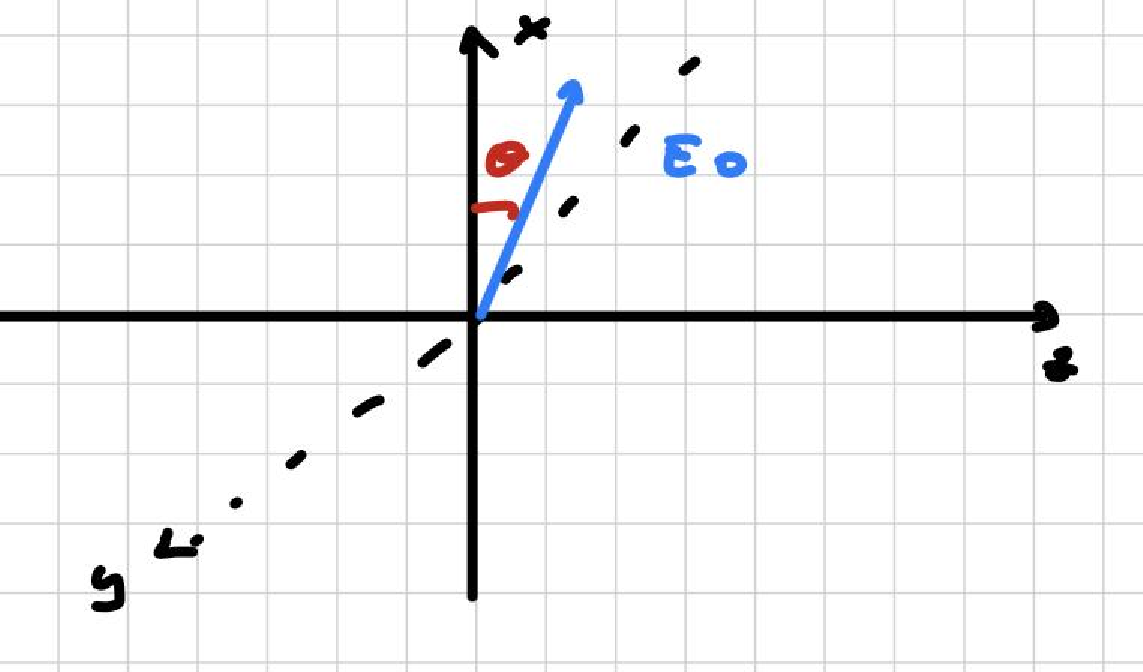
\includegraphics[width=0.8\textwidth]{images_in_pdf/2-/Grafico_5.pdf} 
\end{figure}

$E_z = 0$, since the wave propagates along $\hat{z}$ and the electric field is transverse. The field components can be written as:
\begin{equation}
\begin{cases}
    E_x(z,t) = E_{0,x} \cos(kz - \omega t + \phi_1)\\
    E_y(z,t) = E_{0,y} \cos(kz - \omega t + \phi_2)
\end{cases}
\end{equation}

We parametrize the amplitudes as:
\begin{equation}
\begin{cases}
    E_{0,x} = E_0 \cos\theta\\
    E_{0,y} = E_0 \sin\theta
\end{cases}
\end{equation}

Using the complex representation $\left(\cos\alpha = \Re\{{e^{i\alpha}}\}\right)$, the electric field can be written as:
\[
\vec{E}(z,t) = \Re \left\{ E_0 \cdot e^{\phi_1}\cdot  \left( \cos\theta\, \hat{x} + e^{i\Delta\phi}\sin\theta\, \hat{y} \right) e^{i(kz - \omega t)} \right\}
\]
where $\Delta\phi = \phi_2 - \phi_1$ is the relative phase between the two components. The overall phase $e^{\phi_1}$ is not physically relevant.

The vector:
\begin{equation}\label{eqn:2-polarization-vector}
\vec{e}_{\theta,\phi} = \cos\theta\, \hat{x} + e^{i\Delta\phi}\sin\theta\, \hat{y}
\end{equation}

is called the \textbf{polarization vector} and fully characterizes the polarization state of the wave.

Different choices of $\theta$ and $\Delta\phi$ correspond to different polarization states:

\begin{enumerate}
    \item If $\Delta \phi = 0$ (or $\pi$), the field components oscillate in phase and the wave is \textbf{linearly polarized}. In particular:
    \begin{itemize}
        \item $\theta = 0 \Rightarrow$ polarization along $\hat{x}$;
        \item $\theta = \frac{\pi}{2} \Rightarrow$ polarization along $\hat{y}$.
    \end{itemize}
    
    \item If $\theta = \frac{\pi}{4}$ and $\Delta\phi = \pm \frac{\pi}{2}$, the wave is \textbf{circularly polarized}, with polarization vectors:
    \begin{equation}\label{eqn:2-circular-polarization}
        \vec{e}_{\sigma^{\pm}} = \frac{1}{\sqrt{2}}(\hat{x} \pm i \hat{y})
    \end{equation}
    
    \item In the general case, the wave is \textbf{elliptically polarized}.    
\end{enumerate}

\hl{In quantum mechanics, the polarization state of a single photon is described by a two-dimensional complex Hilbert space}. Any polarization state can be written as a superposition of two orthogonal basis states, for example $(\hat{x}, \hat{y})$ or the circular basis. This representation is not unique, but any pair of orthogonal states spans the space.

The key point is that polarization provides a fundamental and controllable degree of freedom, widely used in both classical and quantum optical experiments.